\section{Parsing}

\begin{figure}[h]
    \centering
    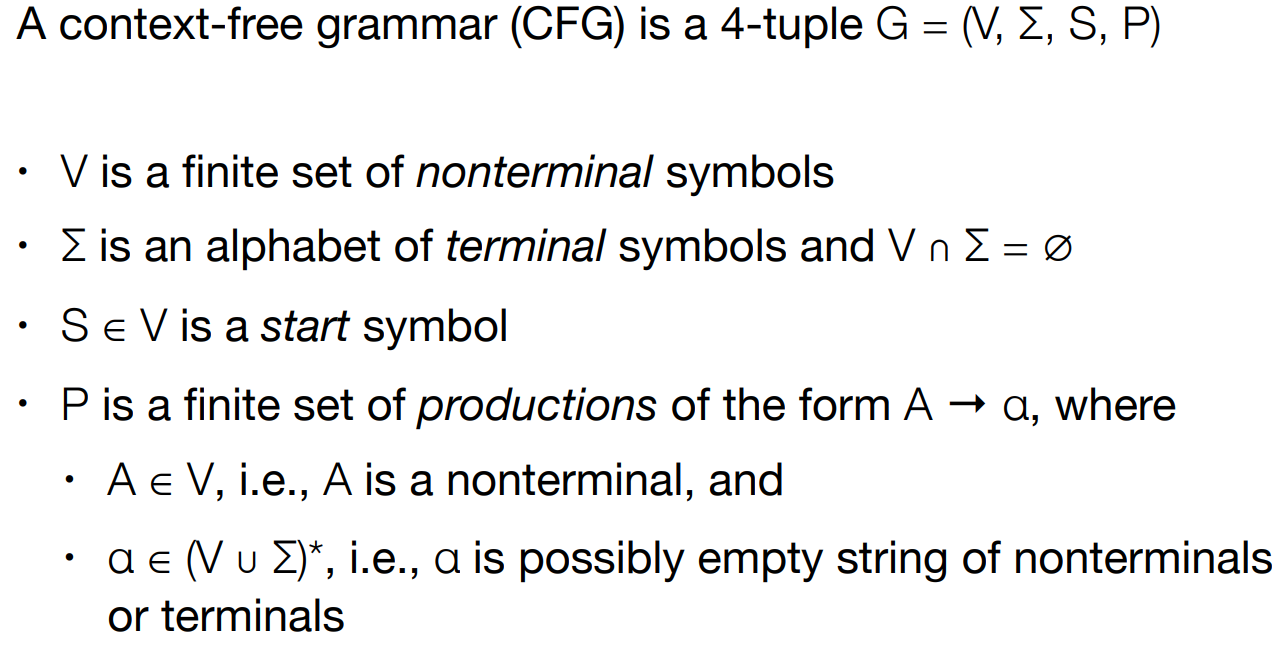
\includegraphics[scale=0.35]{assets/cfg_def.png}
    \caption{CFG Definition}
    \label{fig:cfg}
\end{figure}

\begin{figure}[h]
    \centering
    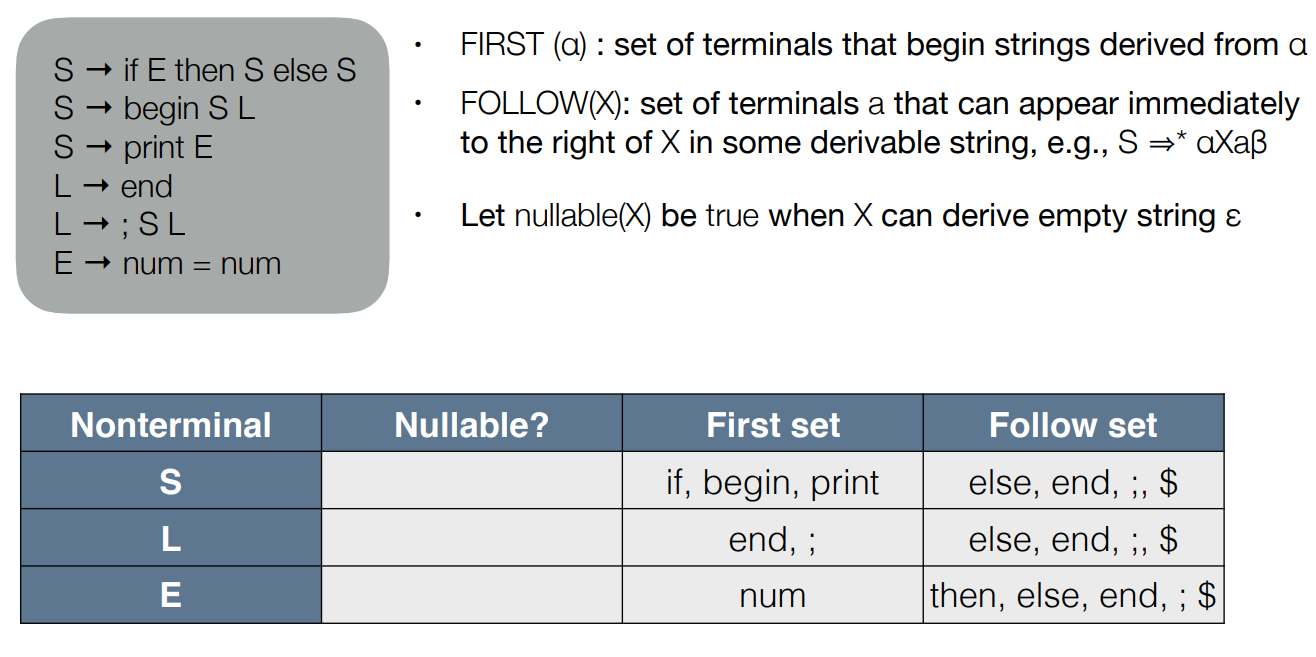
\includegraphics[scale=0.35]{assets/top-down_parsing_table.png}
    \caption{Top-down parsing table. You do not want more than one possibility in a cell.}
    \label{fig:top-down}
\end{figure}

\begin{itemize}
    \item Abstract Syntax Tree (AST): 
    \item Context-Free Grammars (CFG): 
    \begin{itemize}
        \item \textit{Terminals} $\rightarrow$ \textit{production rules}
        \item Terminals are leafs in the tree (e.g. x, y).
        \item Non-Terminals are links in the tree (e.g. BinExp)
        \item Definition see figure \ref{fig:cfg}.
        \item Ambiguity: You don't want ambiguity, you want determinism. \textit{Associativity} (right/left) and \textit{precedence} (e.g. times before plus).
    \end{itemize}
    \item Top-down/Bottom-up parsing:
    \begin{itemize}
        \item Top-down is predictive parsing:
        \begin{itemize}
            \item leftmost derivation
            \item "see whats coming"
            \item Breaks down at for example: $S$ $\rightarrow$ $S+x$ | $S-x$ | $x$. Here you don't know what to do when you see an $x\dots$
            \item See figure \ref{fig:top-down} for parsing table.
        \end{itemize}
        \item Bottom-up: \textbf{LR parsing} is rightmost reduction.
        \begin{itemize}
            \item Rightmost reduction
            \item Includes EOF "\$" symbol.
        \end{itemize}
    \end{itemize}
\end{itemize}

\subsection{LR parsing}

\textbf{Bottom-up}:
\begin{itemize}
    \item Rightmost reduction
    \item Includes EOF "\$" symbol.
\end{itemize}

\textbf{Terms}:
\begin{itemize}
    \item An \textbf{Item} is a hypothesis about sub-derivations: $N$ is hypothesis, $\alpha$ is confirmed to be parsed, $\beta$ is to be confirmed, $N \rightarrow \alpha.\beta$. Notice that it looks like a production rule, but with a dot somewhere in it.
    \item Item is reducible if $\beta$ is empty. The right side of the dot is empty.
    \item $\epsilon$-closure of an item set: add new hypothesis to set if expecting a non-terminal. Accessible steps while doing lambda steps.
    \item Stack based: stack of alternating items sets and derivation trees.
    \item Conflicts: shift/reduce, reduce/reduce. You don't know what to do from one state, when seeing an input symbol.
\end{itemize}

\textbf{Operations}: Look up stack state, and input symbol to get action
\begin{itemize}
    \item Reduce $k$: Pop stack as many times as the number of symbols on the right-hand side of rule $k$. Choose a grammar rule $X \rightarrow A\ B\ C$; pop $C, B, A$ from the top of the stack, and push X onto the stack. If dot is found on the right side of all symbols.
    \item Shift: Advance input one token; push token to stack. Go from one state to another after seeing a terminal input. Move dot one spot.
    \item Goto: Add hypethesis to stack - which sub-derivations we can go to. Goto state (move across edge). Go from one state to another after seeing a non-terminal. Move dot one spot.
\end{itemize}

Goto and shift must preserve the structure of the stack (item set > derivation). \\

\begin{figure}[h]
    \centering
    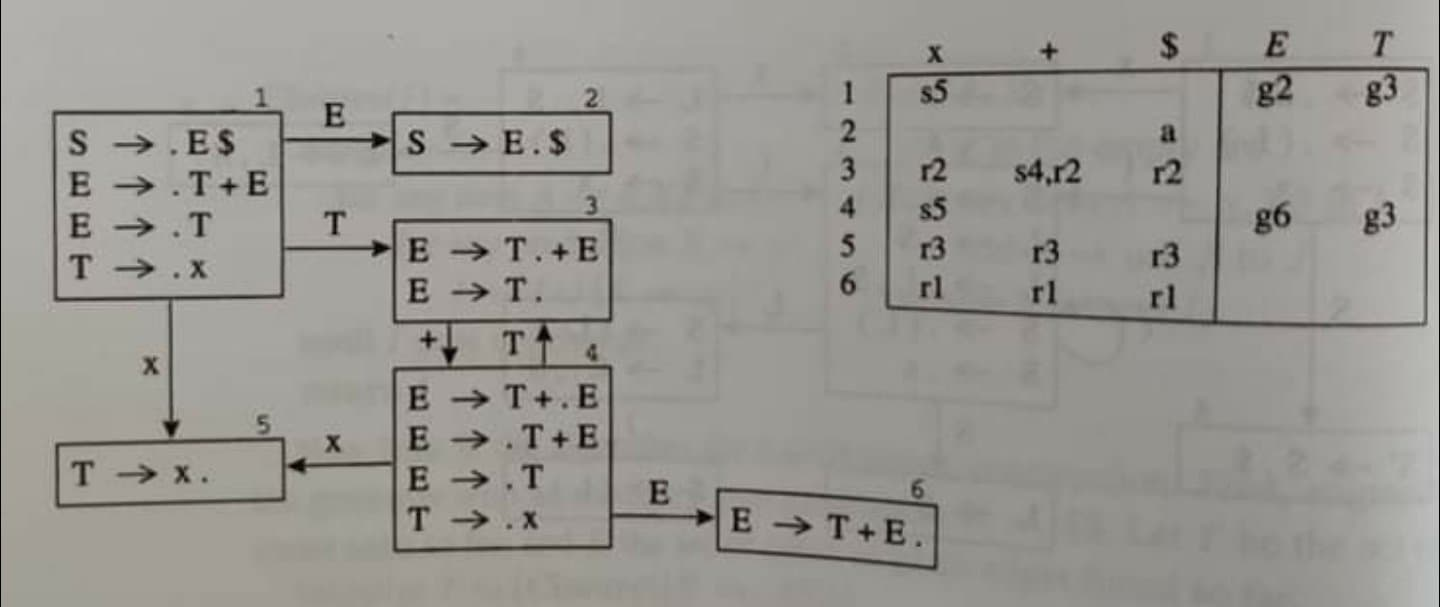
\includegraphics[width=\textwidth]{assets/parsingdfa_table.jpg}
    \caption{LR(0) shift/reduce conflict, parsing table and state DFA, s$n$: shift to state $n$}
    \label{shift/reduce}
\end{figure}

\textbf{Examples}: \href{https://users-cs.au.dk/~askarov/dovs/lr/}{All LR parsing examples}\\

You can create a DFA by calculating first, the starting state and its closure. Then calculate the closures (dot in front of non-terminal) developed by shifting each terminal and non-terminal from that state (moving the dot after the shifted input symbol). Afterwards, you can develop a parsing table, \textit{state} by terminal/non-terminal. See figure \ref{shift/reduce} for parsing table, DFA for shift reduce grammar.\\

Reduction based on $k$ lookahead. The higher $k$, the less conflicts. However, more than 1 is not used for compilation, as the parsing table would be huge.\\

Since LR(0) needs no lookahead, we require one action for each state. With shift and reduce, we get a shift/reduce conflict.\\

LR(1) items consists of a \textit{grammar productio}n, a \textit{right-hand-side position} and a \textit{lookahead symbol}. Choose whether or not to reduce based on stack and one lookahead on input.\\

Lookaheads are calculated by: Any state that contains an item of the form $A \rightarrow x.By\ \{t\}$, where $x$ and $y$ are arbitrary strings of terminals and nonterminals and $B$ is a nonterminal, you add an item of the form $B \rightarrow .w\ \{s\}$ for every production $B \rightarrow w$ and for every terminal in the set $s = FIRST(yt)$.


\subsection{Scoping rules}
Rules of programming language to regulate how names and ID's are resolved.\\

\textbf{Problems}:

\begin{itemize}
    \item Nesting: Same name for variable in nested scopes. What value should we return?
    \item Forward reference: Using something before it is declared. E.g. mutual recursion.
\end{itemize}

\textbf{Scoping terms}:

\begin{itemize}
    \item Scope of declaration: Part of the program where the declaration can be referred to.
    \item \textbf{Static nested scopes (SML style)}: Identifier scope is the smallest block (begin/end, function, or procedure body) containing the identifier's declaration. This means that an identifier declared in some block is only accessible within that block and from procedures declared within it.
    \begin{itemize}
        \item Nearest visible: Return value of nearest declaration in the code.
        \item Stack-like behavior
        \item JS function-level lexical scoping: Inner functions contain the scope of parent functions even if the parent function has returned.
    \end{itemize}
    \item \textbf{Static scoping}: Inner functions can access identifiers in outer scope. Can be deduced in compile time (C).
    \item \textbf{Dynamic scoping}: A function $p$ which prints $x$. Two functions, $d1$ and $d2$,that declare $x$ as 1 and 2 and then calls $p$. $d1$ will print 1 and $d2$ will print 2. I.e. the scope depends on the call stack and chain of function calls.
\end{itemize}

\textbf{Namespace}: Different declaration identifiers can reside in different syntactic namespaces. E.g. in Tiger: \textit{var/function} are in the same namespace, but \textit{type} is in another.

\textbf{Tiger scoping and namespaces}:
\begin{itemize}
    \item Global: base types (\texttt{int}, \texttt{string}) and built-in functions (e.g. \texttt{print}).
\end{itemize}


